

\tikzset{every picture/.style={line width=0.75pt}} %set default line width to 0.75pt

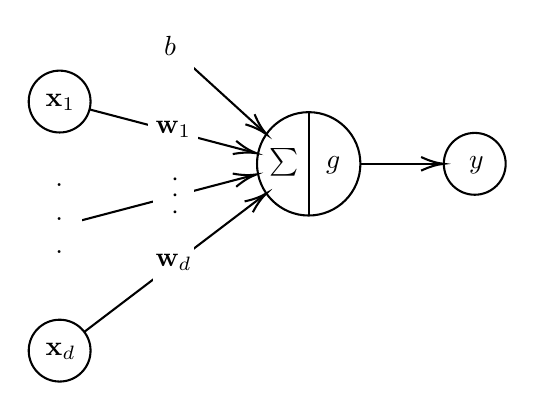
\begin{tikzpicture}[x=0.75pt,y=0.75pt,yscale=-1,xscale=1]
%uncomment if require: \path (0,221); %set diagram left start at 0, and has height of 221

%Shape: Circle [id:dp4208722645887415]
\draw  [fill={rgb, 255:red, 255; green, 255; blue, 255 }  ,fill opacity=1 ] (130.3,85.1) .. controls (130.3,71.35) and (141.45,60.2) .. (155.2,60.2) .. controls (168.95,60.2) and (180.1,71.35) .. (180.1,85.1) .. controls (180.1,98.85) and (168.95,110) .. (155.2,110) .. controls (141.45,110) and (130.3,98.85) .. (130.3,85.1) -- cycle ;
%Straight Lines [id:da3415219367899356]
\draw    (155.2,60.2) -- (155.2,110) ;
%Straight Lines [id:da689750204277868]
\draw    (90,30) -- (133.52,69.65) ;
\draw [shift={(135,71)}, rotate = 222.34] [color={rgb, 255:red, 0; green, 0; blue, 0 }  ][line width=0.75]    (10.93,-3.29) .. controls (6.95,-1.4) and (3.31,-0.3) .. (0,0) .. controls (3.31,0.3) and (6.95,1.4) .. (10.93,3.29)   ;
%Straight Lines [id:da7819738961167022]
\draw    (35.2,175.1) -- (133.41,100.41) ;
\draw [shift={(135,99.2)}, rotate = 502.75] [color={rgb, 255:red, 0; green, 0; blue, 0 }  ][line width=0.75]    (10.93,-3.29) .. controls (6.95,-1.4) and (3.31,-0.3) .. (0,0) .. controls (3.31,0.3) and (6.95,1.4) .. (10.93,3.29)   ;
%Straight Lines [id:da7513165546337284]
\draw    (35.2,55.1) -- (128.07,79.49) ;
\draw [shift={(130,80)}, rotate = 194.72] [color={rgb, 255:red, 0; green, 0; blue, 0 }  ][line width=0.75]    (10.93,-3.29) .. controls (6.95,-1.4) and (3.31,-0.3) .. (0,0) .. controls (3.31,0.3) and (6.95,1.4) .. (10.93,3.29)   ;
%Straight Lines [id:da6597094735122764]
\draw    (35.2,115.1) -- (128.07,90.71) ;
\draw [shift={(130,90.2)}, rotate = 525.28] [color={rgb, 255:red, 0; green, 0; blue, 0 }  ][line width=0.75]    (10.93,-3.29) .. controls (6.95,-1.4) and (3.31,-0.3) .. (0,0) .. controls (3.31,0.3) and (6.95,1.4) .. (10.93,3.29)   ;
%Shape: Circle [id:dp7586847780799892]
\draw  [fill={rgb, 255:red, 255; green, 255; blue, 255 }  ,fill opacity=1 ] (20.3,55.1) .. controls (20.3,46.87) and (26.97,40.2) .. (35.2,40.2) .. controls (43.43,40.2) and (50.1,46.87) .. (50.1,55.1) .. controls (50.1,63.33) and (43.43,70) .. (35.2,70) .. controls (26.97,70) and (20.3,63.33) .. (20.3,55.1) -- cycle ;
%Shape: Circle [id:dp5326237727137924]
\draw  [fill={rgb, 255:red, 255; green, 255; blue, 255 }  ,fill opacity=1 ] (20.3,175.1) .. controls (20.3,166.87) and (26.97,160.2) .. (35.2,160.2) .. controls (43.43,160.2) and (50.1,166.87) .. (50.1,175.1) .. controls (50.1,183.33) and (43.43,190) .. (35.2,190) .. controls (26.97,190) and (20.3,183.33) .. (20.3,175.1) -- cycle ;
%Shape: Rectangle [id:dp3057267797843617]
\draw  [draw opacity=0][fill={rgb, 255:red, 255; green, 255; blue, 255 }  ,fill opacity=1 ] (80,20) -- (100,20) -- (100,40) -- (80,40) -- cycle ;
%Shape: Rectangle [id:dp23384492834953496]
\draw  [draw opacity=0][fill={rgb, 255:red, 255; green, 255; blue, 255 }  ,fill opacity=1 ] (78,58) -- (102,58) -- (102,82) -- (78,82) -- cycle ;
%Shape: Rectangle [id:dp35771934708454767]
\draw  [draw opacity=0][fill={rgb, 255:red, 255; green, 255; blue, 255 }  ,fill opacity=1 ] (26,105) -- (46,105) -- (46,125) -- (26,125) -- cycle ;
%Shape: Rectangle [id:dp586633463938258]
\draw  [draw opacity=0][fill={rgb, 255:red, 255; green, 255; blue, 255 }  ,fill opacity=1 ] (80,125) -- (100,125) -- (100,145) -- (80,145) -- cycle ;
%Shape: Rectangle [id:dp29818210343225005]
\draw  [draw opacity=0][fill={rgb, 255:red, 255; green, 255; blue, 255 }  ,fill opacity=1 ] (80,91) -- (100,91) -- (100,111) -- (80,111) -- cycle ;
%Shape: Circle [id:dp03426447666751509]
\draw  [fill={rgb, 255:red, 255; green, 255; blue, 255 }  ,fill opacity=1 ] (220.3,85.1) .. controls (220.3,76.87) and (226.97,70.2) .. (235.2,70.2) .. controls (243.43,70.2) and (250.1,76.87) .. (250.1,85.1) .. controls (250.1,93.33) and (243.43,100) .. (235.2,100) .. controls (226.97,100) and (220.3,93.33) .. (220.3,85.1) -- cycle ;
%Straight Lines [id:da03800711249960531]
\draw    (180.1,85.1) -- (218.3,85.1) ;
\draw [shift={(220.3,85.1)}, rotate = 180] [color={rgb, 255:red, 0; green, 0; blue, 0 }  ][line width=0.75]    (10.93,-3.29) .. controls (6.95,-1.4) and (3.31,-0.3) .. (0,0) .. controls (3.31,0.3) and (6.95,1.4) .. (10.93,3.29)   ;

% Text Node
\draw (84,22) node [anchor=north west][inner sep=0.75pt]    {$b$};
% Text Node
\draw (80,63) node [anchor=north west][inner sep=0.75pt]    {$\mathbf{w} _{1}$};
% Text Node
\draw (80,127) node [anchor=north west][inner sep=0.75pt]    {$\mathbf{w} _{d}$};
% Text Node
\draw (93,89) node [anchor=north west][inner sep=0.75pt]  [rotate=-90]  {$.\ .\ .$};
% Text Node
\draw (27,50) node [anchor=north west][inner sep=0.75pt]    {$\mathbf{x}_{1}$};
% Text Node
\draw (27,170) node [anchor=north west][inner sep=0.75pt]    {$\mathbf{x}_{d}$};
% Text Node
\draw (135,76) node [anchor=north west][inner sep=0.75pt]    {$\sum $};
% Text Node
\draw (162.1,80) node [anchor=north west][inner sep=0.75pt]    {$g$};
% Text Node
\draw (25,83.5) node [anchor=north west][inner sep=0.75pt]    {$ \begin{array}{l}
.\\
.\\
.
\end{array}$};
% Text Node
\draw (231,80) node [anchor=north west][inner sep=0.75pt]    {$y$};


\end{tikzpicture}